\subsection{Сбор данных (Савосин Артем, Гусев Владислав, Вишневский Глеб, Макаров Максим, Самарин Артем)}
Для работы по обучению модели, классифицирующей жесты, необходимо было собрать данные с этими жестами. Предположив, что жесты пользователей будут различаться в зависимости от их возраста, пола, физических особенностей, было принято решение собрать записи движений разных пользователей. Удалось записать движения 10 пользователей, 6 персон женского пола, 4 мужского, 5 пользователей старшей возрастной группы.

Также был учтен факт использования пользователями жестов с различными количествами тактов(разделение данных по разным группами в зависимостиот количества тактов).

Суммарно мы получили 600 различных движений.
Данные заранее были случайным образом разбиты на две группы - для тренировки модели и для проверки ее точности.

\begin{figure}[H]
    \center{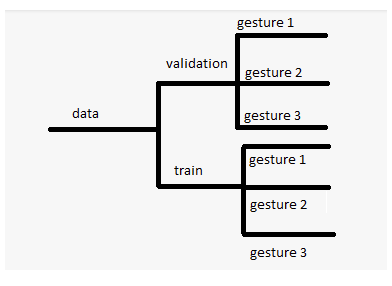
\includegraphics[scale = 1]{images_sav/data.png}}
\end{figure}
